\documentclass[]{article}
\usepackage[utf8]{inputenc}
\usepackage[T1]{fontenc}
\usepackage{graphicx}
\usepackage[portuguese]{babel}

%opening
\title{Projeto POO - Implementação do Pac-Man}
\author{11011716 - André Aranovich Florentino\\ 11003216 - Bruno Tatsuya Masunaga Santos\\ 11076916 - Lucas Eduardo Gonçalves da Rosa\\ 11006216 - Wesley Pereira da Silva}
\date{\today}

\begin{document}

\maketitle

\centerline{\textbf{Turma: A2 - Matutino}}

\section{Introdução}
Este relatório deve conter uma breve descrição do seu projeto, não podendo ultrapassar \textbf{quatro páginas}. Esta seção de introdução deve conter uma descrição sobre o projeto que escolheram implementar e seus objetivos principais. O restante do relatóri deve ser dividido na seguintes seções: Descrição das Classes, Conceitos de Orientação a Objetos Empregados, e Participação dos Integrantes do Grupo, conforme apresentado a seguir. 

\section{Descrição das classes}
Neste projeto, as classes foram criadas com a intenção de implementar a seguinte ideia de modelagem: 

\begin{itemize}
	\item \textbf{GameManager}: É a classe que controla todo o fluxo do jogo. Possui métodos responsáveis pela impressão de movimentação dos elementos ao longo do mapa e de controle de vidas e pontos, além de instanciar todas as demais classes (exceto Principal). De modo geral, é a classe que controla o jogo. 
	\item \textbf{Labirinto}: Responsável por ler um mapa a partir de um arquivo .txt, traduzindo-o para uma matriz. Possui métodos get e set para tratar as células dessa matriz. A intenção é que exista uma instância global e única desta classe no programa.
	\item \textbf{Personagem}: Classe abstrata que representa dois elementos específicos no jogo: o Pac-Man e os fantasmas. Esta classe possui métodos e atributos comuns a essas duas entidades.
	\item \textbf{Pacman}: Estende Personagem e representa a abstração do Pac-Man. Possui alguns métodos sobrescritos que vêm de Personagem e outros que são apenas herdados. Além disso, possui métodos para movimentação do Pac-Man. A intenção é que exista apenas uma instância desta classe no programa (assim como Labirinto).
	\item \textbf{Fantasma}: Estende Personagem e representa a abstração de um fantasma. Assim como a classe Pacman, também sobrescreve e herda determinados métodos de Personagem. Ademais, possui métodos para a movimentação dos fantasmas e para eliminar o Pac-Man. No entanto, diferentemente da classe Pacman, espera-se a existência de várias instâncias de Fantasma no programa.
	\item \textbf{Controle}: Classe responsável por capturar as teclas pressionadas pelo usuário em tempo real. Implementa a classe KeyListener (responsável pelos métodos de captura de entradas) e estende a classe JFrame (que cria uma janela utilizando Swing, sendo responsável por habilitar os métodos de KeyListener). Mais uma vez, a intenção é que haja uma classe única e global no programa.
	\item \textbf{Principal}: Classe onde localiza-se o programa que será executado (main). Instancia um único objeto de GameManager. Possui métodos para escolha do número de fantasmas, do mapa e da dificuldade do jogo, além de habilitar a opção de "Jogar Novamente".
\end{itemize}

Na imagem abaixo, apresenta-se o diagrama UML elaborado. Este diagrama demonstra a modelagem e a relação entre as classes, apresentando os atributos e métodos de cada uma:

\begin{center}
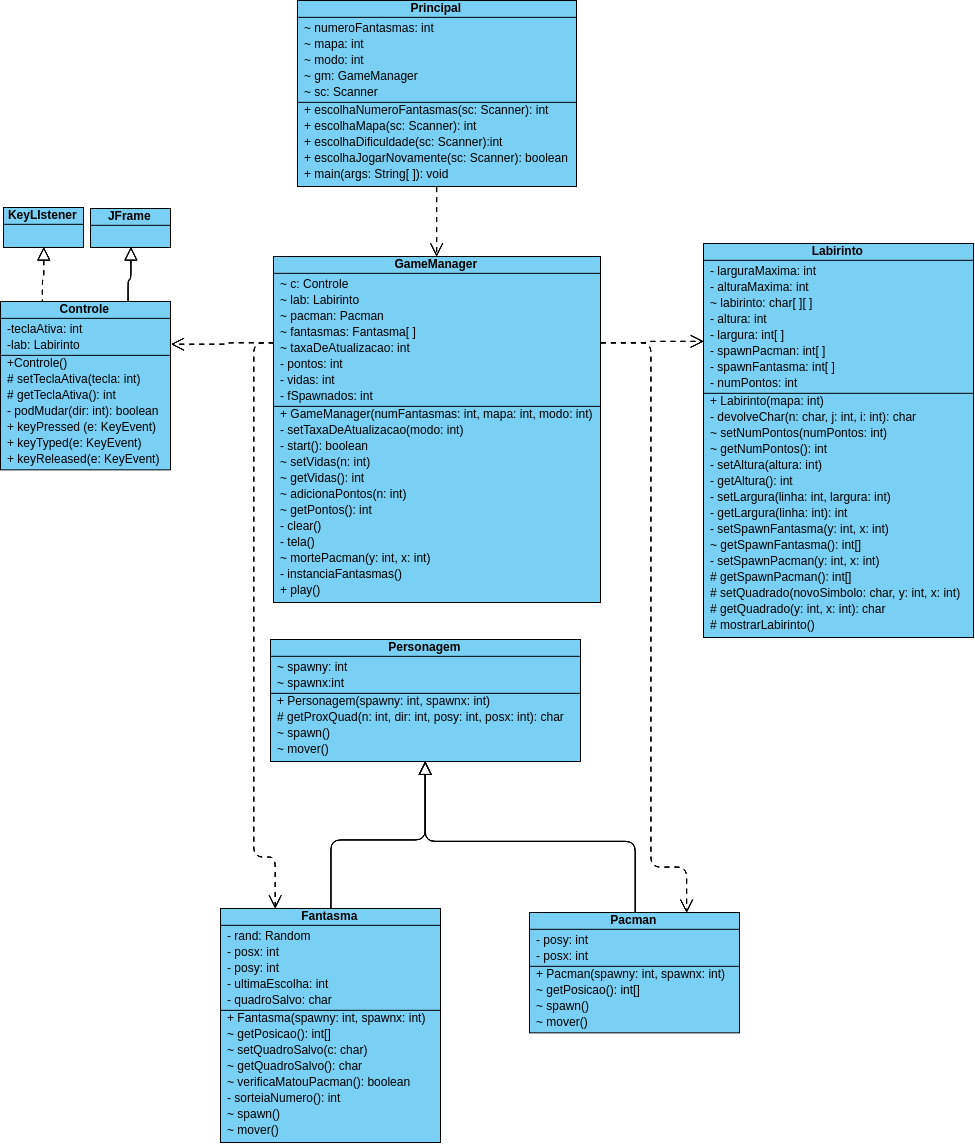
\includegraphics[width=12cm]{UML.PNG}
\end{center}

\section{Conceitos de orientação a objetos aplicados}
Descreva os conceitos de Orientação a Objetos empregados no seu projeto. Se Padrões de Projeto foram implementados, descreva quais foram e como foram usados.

\section{Participação de cada integrante do grupo}
Esta seção deve conter uma descrição da contribuição de cada integrante do grupo para realização do projeto. Por exemplo, descreva quem foi responsável pela implementação de cada classe, quem ficou responsável pela modelagem do sistema, pela confecção do relatório e geração do diagrama de classes.

\end{document}
